\documentclass[aspectratio=169]{beamer}
\usepackage[utf8]{inputenc}
\usepackage{lmodern}
\usepackage{tikz}
\usepackage{hyperref}
\usetikzlibrary{positioning,arrows.meta,calc,shapes.geometric}

\definecolor{accent1}{HTML}{0F766E}
\definecolor{accent2}{HTML}{99F6E4}
\definecolor{accent3}{HTML}{F59E0B}
\definecolor{accent4}{HTML}{134E4A}
\definecolor{paper}{HTML}{F6FFFD}
\definecolor{ink}{HTML}{1F2937}

\setbeamertemplate{navigation symbols}{}
\setbeamercolor{normal text}{fg=ink,bg=white}
\setbeamercolor{frametitle}{fg=ink,bg=white}
\setbeamertemplate{itemize item}{\color{accent1}$\blacktriangleright$}
\setbeamertemplate{enumerate item}{\color{accent1}\insertenumlabel.}
\setbeameroption{hide notes}

\title{Build Shapes with Builderz}
\subtitle{Teacher Presentation}
\author{Pine Brook IGNITE}
\date{Spring 2026}

\begin{document}

\begin{frame}[plain]
\begin{tikzpicture}[remember picture,overlay]
\fill[paper] (current page.south west) rectangle (current page.north east);
\fill[accent1!10] (0.25,0.4) rectangle (13.05,7.0);
\draw[line width=7pt, color=accent3] (0.55,6.75) -- (12.75,6.75);
\draw[line width=7pt, color=accent2] (0.55,0.65) -- (12.75,0.65);
\end{tikzpicture}
\vspace{0.45cm}
\begin{columns}[T,totalwidth=\textwidth]
\column{0.58\textwidth}
{\Huge\bfseries\color{ink} Build Shapes with Builderz\par}
\vspace{0.18cm}
{\Large\color{accent4} Create. Compare. Reflect.\par}
\vspace{0.25cm}
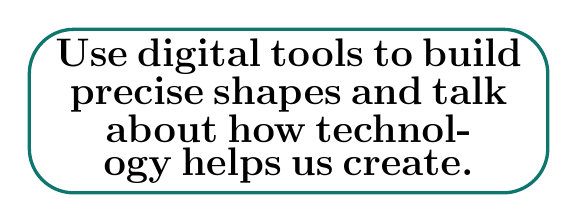
\begin{tikzpicture}
\node[rounded corners=16pt, fill=white, draw=accent1, line width=1.2pt, text width=6.35cm, minimum height=1.4cm, align=center]
{\Large\bfseries Use digital tools to build precise shapes and talk about how technology helps us create.};
\end{tikzpicture}
\vspace{0.35cm}

\begin{tikzpicture}[node distance=0.42cm]
\node[rounded corners=14pt, fill=accent3!16, draw=accent3!80, minimum width=2.3cm, minimum height=1.08cm, align=center] (a) {\Large\bfseries 1\\[2pt]Notice};
\node[rounded corners=14pt, fill=accent2!18, draw=accent2!85!black, minimum width=2.3cm, minimum height=1.08cm, align=center, right=of a] (b) {\Large\bfseries 2\\[2pt]Build};
\node[rounded corners=14pt, fill=accent1!14, draw=accent1!80!black, minimum width=2.3cm, minimum height=1.08cm, align=center, right=of b] (c) {\Large\bfseries 3\\[2pt]Share};
\end{tikzpicture}
\column{0.36\textwidth}
\begin{center}
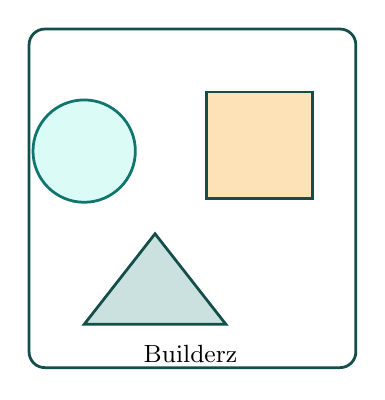
\begin{tikzpicture}[x=1cm,y=1cm]
\draw[rounded corners=0.2cm, fill=white, draw=accent4, line width=1pt] (0.3,0.45) rectangle (4.45,4.75);
\draw[fill=accent2!35, draw=accent1, line width=1pt] (1.0,3.2) circle (0.65);
\draw[fill=accent3!30, draw=accent4, line width=1pt] (2.55,2.6) rectangle (3.9,3.95);
\draw[fill=accent1!22, draw=accent4, line width=1pt] (1.0,1.0) -- (1.9,2.15) -- (2.8,1.0) -- cycle;
\node[align=center] at (2.35,0.62) {\small Builderz};
\end{tikzpicture}
\end{center}
\end{columns}
\note{Open by naming the goal in student-friendly language and previewing the routine: notice shapes, build with the tool, then share what worked.}
\end{frame}

\begin{frame}[plain]
\frametitle{Today's Learning Goal}
\begin{columns}[T,totalwidth=\textwidth]
\column{0.56\textwidth}
\begin{block}{I can statement}
\large I can use Builderz to make shapes and explain how a digital tool helps me create more carefully.
\end{block}
\vspace{0.15cm}
\begin{itemize}
\large
\item I can build a circle and other simple shapes.
\item I can compare making shapes by hand and on a Chromebook.
\item I can explain one thing I noticed about accuracy or ease.
\end{itemize}
\column{0.38\textwidth}
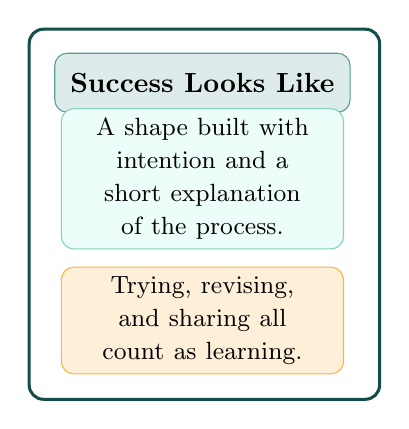
\begin{tikzpicture}[x=1cm,y=1cm]
\draw[rounded corners=0.18cm, fill=white, draw=accent4, line width=1.1pt] (0.1,0.1) rectangle (4.55,4.8);
\node[rounded corners=0.16cm, fill=accent1!14, draw=accent1!70, minimum width=3.75cm, minimum height=0.75cm, align=center] at (2.3,4.12) {\bfseries Success Looks Like};
\node[rounded corners=0.16cm, fill=accent2!18, draw=accent2!85!black, text width=3.35cm, minimum height=1.15cm, align=center] at (2.3,2.9) {\small A shape built with intention and a short explanation of the process.};
\node[rounded corners=0.16cm, fill=accent3!16, draw=accent3!75, text width=3.35cm, minimum height=1.0cm, align=center] at (2.3,1.1) {\small Trying, revising, and sharing all count as learning.};
\end{tikzpicture}
\end{columns}
\note{Keep the objective concrete: precision, comparison, and reflection.}
\end{frame}

\begin{frame}[plain]
\frametitle{Application Activity}
\begin{block}{Teacher model}
\large Open \texttt{drawings.new}, try the Pen tool to make a circle, then wonder aloud whether the circle shape tool might help us draw a more perfect shape.
\end{block}
\vspace{0.2cm}
\begin{enumerate}
\large
\item Students open \texttt{drawings.new}.
\item Students experiment with Builderz or the drawing tools to create a perfect circle.
\item Students keep building with other simple shapes if they finish early.
\item Teacher sets a visible timer and encourages revision.
\end{enumerate}
\vspace{0.2cm}
\begin{block}{Teacher language}
\large ``Your job is not to be fast. Your job is to test tools, notice what happens, and improve your shape.''
\end{block}
\note{This slide mirrors the lesson guide sequence and gives you a ready-to-say line that supports productive struggle.}
\end{frame}

\begin{frame}[plain]
\frametitle{Build Shapes Challenge}
\begin{columns}[T,totalwidth=\textwidth]
\column{0.54\textwidth}
\begin{itemize}
\large
\item First, make one circle you are proud of.
\item Next, build two more perfect shapes.
\item Then, combine shapes to make a picture, design, or object.
\item Save your work so you can talk about one smart choice you made.
\end{itemize}
\column{0.4\textwidth}
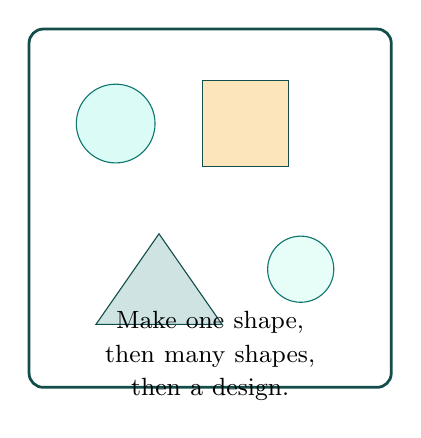
\begin{tikzpicture}[x=1cm,y=1cm]
\draw[rounded corners=0.18cm, fill=white, draw=accent4, line width=1pt] (0.15,0.2) rectangle (4.75,4.75);
\draw[fill=accent2!35, draw=accent1] (1.25,3.55) circle (0.5);
\draw[fill=accent3!28, draw=accent4] (2.35,3.0) rectangle (3.45,4.1);
\draw[fill=accent1!20, draw=accent4] (1.0,1.0) -- (1.8,2.15) -- (2.6,1.0) -- cycle;
\draw[fill=accent2!25, draw=accent1] (3.6,1.7) circle (0.42);
\node[text width=3.7cm, align=center] at (2.45,0.6) {\small Make one shape, then many shapes, then a design.};
\end{tikzpicture}
\end{columns}
\note{Offer extension inside the same activity so early finishers stay engaged without needing a separate transition.}
\end{frame}

\begin{frame}[plain]
\frametitle{Inclusion and Support Moves}
\begin{itemize}
\large
\item Model each step visually before students begin.
\item Keep directions chunked: open, choose a tool, make one shape, revise.
\item Offer flexible participation: mouse, trackpad, touchpad helper, or verbal coach.
\item Pair students strategically so talk supports problem solving.
\item Provide sentence frames such as ``I used \_\_\_ because \_\_\_.'' and ``This tool helped me make a more \_\_\_ shape.''
\item Celebrate revision, not just neat final products.
\end{itemize}
\vspace{0.18cm}
\begin{block}{Accessibility reminder}
\large Students may demonstrate understanding by showing the shape, explaining their process aloud, or comparing hand-drawn and digital work.
\end{block}
\note{This slide makes inclusion explicit and supports multilingual learners, students with fine-motor needs, and students who benefit from oral language scaffolds.}
\end{frame}

\begin{frame}[plain]
\frametitle{CS Standards Connection}
\begin{block}{Aligned CSTA K--2 ideas}
\begin{itemize}
\large
\item \textbf{1A-AP-08}: Model daily processes by creating and following steps to complete a task.
\item \textbf{1A-AP-12}: Develop plans that describe a program's sequence of events, goals, and outcomes.
\item \textbf{1A-IC-17}: Work respectfully and responsibly with others when using computing technologies.
\end{itemize}
\end{block}
\vspace{0.18cm}
\begin{block}{How this lesson supports the standards}
\large Students follow a sequence to open a tool, choose features, create shapes, revise their work, and discuss how digital tools change the outcome.
\end{block}
\note{Use this frame if you need standards language for observation, planning, or administrator-facing materials.}
\end{frame}

\begin{frame}[plain]
\frametitle{Closure: Group Share}
\begin{columns}[T,totalwidth=\textwidth]
\column{0.52\textwidth}
\begin{block}{Discussion prompts}
\begin{itemize}
\large
\item Were you able to draw a circle using your Chromebook?
\item What did you like about drawing a circle with pencil and paper?
\item What did you like about drawing a circle with your Chromebook?
\end{itemize}
\end{block}
\column{0.42\textwidth}
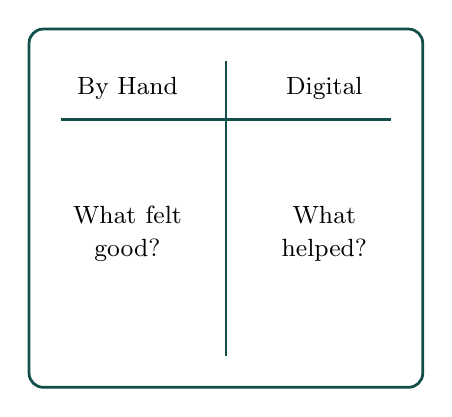
\begin{tikzpicture}[x=1cm,y=1cm]
\draw[rounded corners=0.18cm, fill=white, draw=accent4, line width=1pt] (0.0,0.15) rectangle (5.0,4.7);
\draw[accent4, line width=1pt] (2.5,0.55) -- (2.5,4.3);
\draw[accent4, line width=1pt] (0.4,3.55) -- (4.6,3.55);
\node at (1.25,3.95) {\small By Hand};
\node at (3.75,3.95) {\small Digital};
\node[text width=1.7cm, align=center] at (1.25,2.1) {\small What felt good?};
\node[text width=1.7cm, align=center] at (3.75,2.1) {\small What helped?};
\end{tikzpicture}
\end{columns}
\vspace{0.18cm}
\begin{block}{Teacher move}
\large Record ideas on a t-chart or Venn diagram to help students compare both experiences.
\end{block}
\note{The comparison talk is the learning evidence here, not just the finished drawing.}
\end{frame}

\begin{frame}[plain]
\frametitle{Extension and Spaced Practice}
\begin{itemize}
\large
\item Show students simple pictures made from circles, squares, triangles, and rectangles.
\item Ask them to recreate the image by hand and then with Builderz or Google Drawings shape tools.
\item Invite reflection: What felt easier by hand? What felt easier with technology?
\item Revisit shape-building during center time, morning work, or art integration to strengthen retention.
\end{itemize}
\vspace{0.22cm}
\begin{block}{Exit idea}
\large ``One way technology helped me today was \_\_\_. One way I still want to improve is \_\_\_.'' 
\end{block}
\note{This extension keeps the concept alive across subjects and helps students internalize when digital precision tools are useful.}
\end{frame}

\end{document}
